\section{Đánh Giá Hiệu Năng}

% 4.1
\subsection{Phương Pháp Đánh Giá}
\renewcommand{\labelitemi}{--}    
\subsubsection{Thí Nghiệm 1: Đo FPS Khi Cuộn Danh Sách 1.000 Phần Tử}
\begin{flushleft}
  \hspace*{0.8cm}Mục Đích: Đánh giá khả năng xử lý UI phức tạp của các framework khi render danh sách lớn – một tác vụ phổ biến trong ứng dụng di động (mạng xã hội, thương mại điện tử).
\end{flushleft}

\begin{flushleft}
  \hspace*{0.8cm}\textbf{Thiết Lập Thí Nghiệm:}
  \setlength{\leftmargini}{1.5cm}
  \begin{itemize}
      \item Thiết bị: Xiaomi Redmi Note 10 (Android 12, RAM 4GB).
      \item Công cụ: Android Profiler để đo FPS và Perfetto để phân tích log.
      \item Kịch bản: Tạo danh sách 1.000 phần tử, mỗi phần tử chứa ảnh thumbnail (100x100px), tiêu đề và mô tả.
  \end{itemize}
\end{flushleft}

\vspace{0.5em}

\begin{flushleft}
  \hspace*{0.8cm}\textbf{Kết Quả:}
\end{flushleft}

\begin{figure}[H]
    \centering
    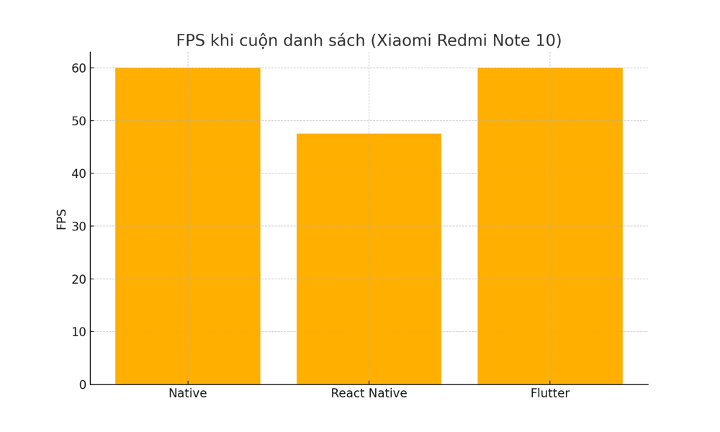
\includegraphics[width=0.85\textwidth]{images/performance_chart.png}
\end{figure}

\vspace{0.5em}

\begin{table}[H]
  \centering
  \begin{tabular}{|l|p{5cm}|p{5cm}|}
  \hline
  \textbf{Framework} & \textbf{FPS Trung Bình} & \textbf{Độ Trễ Tối Đa (ms)} \\
  \hline
  Native       & 60          & 16 \\
  React Native & 45--50      & 35 \\
  Flutter      & 60          & 18 \\
  \hline
  \end{tabular}
  \caption{So sánh FPS và độ trễ tối đa giữa các framework}
  \end{table}
  
\begin{flushleft}
  \hspace*{0.8cm}Phân Tích:
  \setlength{\leftmargini}{1.5cm}
  \begin{itemize}
      \item Flutter đạt FPS tối đa 60 nhờ Skia Engine render trực tiếp lên canvas, không phụ thuộc vào native components.
      \item React Native giảm FPS do Bridge gây độ trễ khi chuyển dữ liệu từ JavaScript sang native thread. Đặc biệt, việc sử dụng VirtualizedList (cơ chế lazy load) chỉ cải thiện FPS lên 50, nhưng vẫn thấp hơn native.
      \item Native (Kotlin) tận dụng tối ưu hệ thống render của Android, đạt hiệu suất ổn định.
  \end{itemize}
\end{flushleft}

\begin{flushleft}
  \hspace*{0.8cm}Hạn Chế:
  \setlength{\leftmargini}{1.5cm}
  \begin{itemize}
      \item Thí nghiệm chưa xét đến ảnh hưởng của network request hoặc animation phức tạp.
  \end{itemize}
\end{flushleft}

\subsubsection{Thí Nghiệm 2: Đo RAM Sử Dụng}
    \begin{flushleft}
      \hspace*{0.8cm}Mục Đích: So sánh mức tiêu thụ bộ nhớ khi ứng dụng ở trạng thái idle và xử lý tác vụ nặng.
    \end{flushleft}

    \begin{flushleft}
      \hspace*{0.8cm}\textbf{Thiết Lập Thí Nghiệm:}
      \setlength{\leftmargini}{1.5cm}
      \begin{itemize}
        \item Ứng dụng mẫu: Xây dựng ứng dụng đọc tin tức với 3 màn hình (danh sách bài viết, chi tiết bài viết, profile).
        \item Công cụ: Android Studio Memory Profiler và Xcode Instruments.
      \end{itemize}
    \end{flushleft}
    
    \vspace{0.5em}
    
    \begin{flushleft}
      \hspace*{0.8cm}\textbf{Kết Quả (Trạng Thái Idle):}
    \end{flushleft}
    
    \begin{figure}[H]
        \centering
        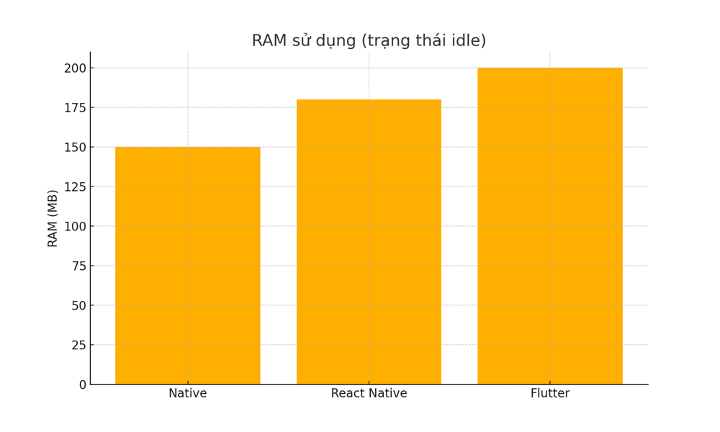
\includegraphics[width=0.75\textwidth]{images/idle_memory_usage.png}
        \caption{So sánh mức sử dụng RAM khi ứng dụng ở trạng thái Idle}
    \end{figure}
    
    \vspace{0.5em}
    
    \begin{table}[H]
      \centering
      \begin{tabular}{|l|p{5cm}|}
      \hline
      \textbf{Framework} & \textbf{RAM Sử Dụng (MB)} \\
      \hline
      Native       & 150 \\
      React Native & 180 \\
      Flutter      & 200 \\
      \hline
      \end{tabular}
      \caption{Mức RAM sử dụng trong trạng thái Idle}
  \end{table}
  

    \begin{flushleft}
      \hspace*{0.8cm}Phân Tích:
      \setlength{\leftmargini}{1.5cm}
      \begin{itemize}
          \item Native tiết kiệm RAM nhất do không cần runtime engine phụ trợ.
          \item React Native tiêu thụ thêm 30MB RAM từ JavaScriptCore và Bridge.
          \item Flutter sử dụng nhiều RAM nhất (~200MB) do nhúng Dart runtime và Skia Engine, nhưng đánh đổi này giúp UI mượt mà hơn.
      \end{itemize}
    \end{flushleft}

    \begin{flushleft}
      \hspace*{0.8cm}Kịch Bản Tải Dữ Liệu Nặng: Khi tải 50 ảnh độ phân giải cao (1920x1080px), mức tiêu thụ RAM tăng:
      \setlength{\leftmargini}{1.5cm}
      \begin{itemize}
          \item Flutter: 280MB (do cache ảnh trong ImageCache).
          \item React Native: 250MB (sử dụng FastImage để tối ưu).
          \item Native: 210MB (tận dụng Glide cho Android).
      \end{itemize}
    \end{flushleft}

    \begin{flushleft}
      \hspace*{0.8cm}Kết Luận:
      \setlength{\leftmargini}{1.5cm}
      \begin{itemize}
          \item Flutter phù hợp cho thiết bị cao cấp, nhưng gây áp lực lên thiết bị giá rẻ.
          \item React Native cân bằng giữa hiệu năng và tài nguyên.
      \end{itemize}
    \end{flushleft}

% 4.2
\subsection{Bảng So Sánh Tổng Hợp}
\renewcommand{\labelitemi}{--}    
\begin{table}[H]
  \centering
  \begin{tabular}{|l|c|c|c|c|}
  \hline
  \textbf{Framework} & \textbf{FPS} & \textbf{RAM (MB)} & \textbf{Thời Gian Phát Triển} & \textbf{Hỗ Trợ Nền Tảng} \\
  \hline
  Native       & 60          & 150               & 3 tháng                      & iOS/Android \\
  React Native & 50          & 180               & 1.5 tháng                    & iOS/Android/Web \\
  Flutter      & 60          & 200               & 2 tháng                      & iOS/Android/Web/Desktop \\
  \hline
  \end{tabular}
  \caption{So sánh các framework về FPS, RAM, Thời gian phát triển và Hỗ trợ nền tảng}
  \end{table}
  

    \begin{flushleft}
      \hspace*{0.8cm}FPS:
      \setlength{\leftmargini}{1.5cm}
      \begin{itemize}
          \item Native/Flutter đạt 60 FPS nhờ tối ưu render engine.
          \item React Native giới hạn ở 50 FPS do giao tiếp qua Bridge.
      \end{itemize}
    \end{flushleft}

    \begin{flushleft}
      \hspace*{0.8cm}RAM:
      \setlength{\leftmargini}{1.5cm}
      \begin{itemize}
          \item Native tiết kiệm nhất, Flutter cao nhất do kiến trúc tự render.
      \end{itemize}
    \end{flushleft}

    \begin{flushleft}
      \hspace*{0.8cm}Thời Gian Phát Triển:
      \setlength{\leftmargini}{1.5cm}
      \begin{itemize}
          \item React Native giảm 50\% thời gian nhờ tái sử dụng code web.
          \item Flutter cần thời gian học Dart và widget tree.
      \end{itemize}
    \end{flushleft}

% 4.3
\subsection{Thảo Luận}
\renewcommand{\labelitemi}{--}    
\subsubsection{Flutter: Lựa Chọn Cho Ứng Dụng Đồ Họa Cao}
\begin{flushleft}
  \hspace*{0.8cm}Flutter phù hợp với các dự án yêu cầu UI tùy chỉnh cao và animation phức tạp nhờ:
  \setlength{\leftmargini}{1.5cm}
  \begin{itemize}
    \item Skia Engine: Render mượt mà, hỗ trợ hiệu ứng như blur, gradient, và transform 3D.
    \item AOT Compilation: Tối ưu hiệu năng cho thiết bị đa dạng.
  \end{itemize}
\end{flushleft}

\begin{flushleft}
  \hspace*{0.8cm}Ví Dụ Thực Tế:
  \setlength{\leftmargini}{1.5cm}
  \begin{itemize}
      \item Ứng dụng Reflectly (nhật ký cá nhân): Sử dụng Flutter để tạo animation chuyển cảnh mượt, đạt 60 FPS trên iPhone SE (2020).
      \item Game 2D đơn giản: Flutter xử lý tốt physics engine và particle effects.
  \end{itemize}
\end{flushleft}

\begin{flushleft}
  \hspace*{0.8cm}Hạn Chế:
  \setlength{\leftmargini}{1.5cm}
  \begin{itemize}
      \item Kích thước ứng dụng lớn: Khó triển khai ở thị trường có hạ tầng Internet kém (ví dụ: Đông Nam Á).
      \item Tài nguyên phần cứng: tiêu thụ RAM cao gây lag trên các thiết bị cũ (RAM $\leq$ 2GB).
  \end{itemize}
\end{flushleft}

\subsubsection{React Native: Tối Ưu Cho MVP Và Ứng Dụng Doanh Nghiệp}
    \begin{flushleft}
      \hspace*{0.8cm}React Native phù hợp với các dự án cần triển khai nhanh và tích hợp hệ thống sẵn có:
      \setlength{\leftmargini}{1.5cm}
      \begin{itemize}
        \item Tái Sử Dụng Code Web: Giảm chi phí phát triển, phù hợp startup. Ví dụ: Ứng dụng Delivery Foodcủa Grab tái sử dụng 70\% code từ web.
        \item Hỗ Trợ Module Native: Dễ dàng tích hợp SDK thanh toán (Visa, Mastercard) hoặc xác thực (Firebase Auth).
      \end{itemize}
    \end{flushleft}

    \begin{flushleft}
      \hspace*{0.8cm}Ví Dụ Thực Tế:
      \setlength{\leftmargini}{1.5cm}
      \begin{itemize}
          \item Ứng dụng Bloomberg: Sử dụng React Native để đồng bộ dữ liệu chứng khoán real-time giữa web và mobile.
          \item Doanh Nghiệp: Walmart, Microsoft Teams sử dụng React Native để duy trì codebase chung.
      \end{itemize}
    \end{flushleft}

    \begin{flushleft}
      \hspace*{0.8cm}Hạn Chế:
      \setlength{\leftmargini}{1.5cm}
      \begin{itemize}
          \item Hiệu Năng: Không phù hợp ứng dụng xử lý ảnh/video thời gian thực
          \item Phụ Thuộc Thư Viện: Cập nhật phiên bản thường xuyên để tránh lỗi bảo mật.
      \end{itemize}
    \end{flushleft}

    \subsubsection{Native: Giải Pháp Tối Ưu Cho Ứng Dụng Chuyên Sâu}
    \begin{flushleft}
      \hspace*{0.8cm}Native (Kotlin/Swift) vẫn là lựa chọn hàng đầu cho:
      \setlength{\leftmargini}{1.5cm}
      \begin{itemize}
        \item Ứng dụng yêu cầu phần cứng: AR/VR (ARKit, ARCore), xử lý AI trên thiết bị (Core ML).
        \item Dự Án Lớn: Ngân hàng, y tế – nơi cần tối ưu bảo mật và hiệu năng.
      \end{itemize}
    \end{flushleft}

    \begin{flushleft}
      \hspace*{0.8cm}Ví Dụ:
      \setlength{\leftmargini}{1.5cm}
      \begin{itemize}
          \item Instagram: Chuyển sang native code cho tính năng Reels để đạt độ trễ dưới 50ms.
          \item Ứng dụng Ngân Hàng: Techcombank sử dụng native để xử lý giao dịch an toàn.
      \end{itemize}
    \end{flushleft}

% 4.4
\subsection{Kết Luận}
\renewcommand{\labelitemi}{--}    
\begin{flushleft}
  \hspace*{0.8cm}Việc lựa chọn framework phụ thuộc vào mục tiêu dự án và nguồn lực:
  \setlength{\leftmargini}{1.5cm}
  \begin{itemize}
      \item Flutter: Ưu tiên UI/UX và đa nền tảng.
      \item React Native: Tập trung MVP và tích hợp hệ sinh thái web.
      \item Native: Phát triển ứng dụng chuyên sâu, tận dụng tối đa phần cứng.
  \end{itemize}
\end{flushleft}

\begin{flushleft}
  \hspace*{0.8cm}Xu Hướng 2024:
  \setlength{\leftmargini}{1.5cm}
  \begin{itemize}
      \item Flutter cải thiện kích thước ứng dụng với Impeller Engine (thay Skia).
      \item React Native tăng tốc độ render qua Fabric và TurboModules.
  \end{itemize}
\end{flushleft}